\documentclass[11pt]{article}
\usepackage{a4, fullpage}
\usepackage{bibtopic}
\usepackage[small,compact]{titlesec}
\usepackage{float}
\usepackage{amssymb,amsmath}
\usepackage[T1]{fontenc}
\usepackage{graphicx}
\usepackage{multicol}
\restylefloat{table}
%\usepackage{parskip}
%\usepackage{setspace}



\setlength{\parskip}{0.3cm}(where appropriate)
\setlength{\parindent}{0cm}
\setlength{\textheight}{10in}
\setlength{\textwidth}{6.5in}
\setlength{\parskip}{2pt}
\addtolength{\oddsidemargin}{-.3in}
\addtolength{\evensidemargin}{-.3in}
\addtolength{\topmargin}{-.6in}
\addtolength{\textwidth}{.6in}



\begin{document}


\title{Assignment 3 \\ Group 30  }

\author{John Walker \and Adam Fiksen \and Giovanni Charles }

\date{\today}         % inserts today's date

\maketitle           % generates the title from the data above


\section{Results}
% Confuction matrices (for both types of networks)
% Average classification rate and recall, precision and F1 measures per class (part VIII).

\subsection{Confusion Matricies}

\begin{table}[H]
\caption{Confusion Six output Network} % title of Table
\centering % used for centering table
\begin{tabular}{c c c c c c} % centered columns (4 columns)
\hline % inserts single horizontal line
90  & 12   & 4   & 1     & 12  & 1   \\ % inserting body of the table
16  & 169  & 4   & 8     & 24  & 1   \\
5   & 0    & 93  & 1     & 4   & 7   \\
3   & 5    & 1   & 201   & 4   & 2   \\
13  & 12   & 3   & 2     & 86  & 3   \\ 
4   & 0    & 13  & 2     & 2   & 192 \\ [1ex] % [1ex] adds vertical space
\hline %inserts single line
\end{tabular}
\label{table:sixconf} % is used to refer this table in the text
\end{table}

\begin{table}[H]
\caption{Confusion Single Output Networks} % title of Table
\centering % used for centering table
\begin{tabular}{c c c c c c} % centered columns (4 columns)
\hline % inserts single horizontal line
98  & 13   & 4   & 0    & 11  & 1   \\ % inserting body of the table
14  & 164  & 4   & 9    & 16  & 1   \\
3   & 1    & 96  & 0    & 4   & 13  \\
3   & 6    & 1   & 204  & 3   & 3   \\
12  & 14   & 3   & 1    & 95  & 1   \\ 
1   & 0    & 10  & 1    & 3   & 187 \\ [1ex] % [1ex] adds vertical space
\hline %inserts single line
\end{tabular}
\label{table:singconf} % is used to refer this table in the text
\end{table}

\subsection{Average Classification Rate, Recall Precision and F1 Measures}

\begin{table}[H]
\caption{Six Output Evaluation Results} % title of Table
\centering % used for centering table
\begin{tabular}{c c c c c} % centered columns (4 columns)
\hline\hline %inserts double horizontal lines
Emotion & name & Precision rate & Recall rate & f1 measure\\ [0.5ex] % inserts table
\hline % inserts single horizontal line
1 & anger     & 68.7023 & 75.0000 & 70.7131\\ % inserting body of the table
2 & disgust   & 85.3535 & 76.1261 & 80.4762\\
3 & fear      & 78.8136 & 84.5455 & 81.5789\\
4 & happiness & 93.4884 & 93.0556 & 93.2715\\
5 & sadness   & 65.1515 & 72.2689 & 68.5259\\ 
6 & suprise   & 93.2039 & 90.1408 & 91.6468\\ [1ex] % [1ex] adds vertical space
\hline %inserts single line
\end{tabular}
\label{table:sixevaluation} % is used to refer this table in the text
\end{table}

Classification Rate: 0.8310

\begin{table}[H]
\caption{Single Output Evaluation Results} % title of Table
\centering % used for centering table
\begin{tabular}{c c c c c} % centered columns (4 columns)
\hline\hline %inserts double horizontal lines
Emotion & name & Precision rate & Recall rate & f1 measure\\ [0.5ex] % inserts table
\hline % inserts single horizontal line
1 & anger     & 74.8092 & 77.1654 & 75.9690\\ % inserting body of the table
2 & disgust   & 82.8283 & 78.8462 & 80.7882\\
3 & fear      & 81.3559 & 82.0513 & 81.7021\\
4 & happiness & 94.8837 & 92.7273 & 93.7931\\
5 & sadness   & 71.9697 & 75.3968 & 73.6434\\ 
6 & suprise   & 90.7767 & 92.5743 & 91.6667\\ [1ex] % [1ex] adds vertical space
\hline %inserts single line
\end{tabular}
\label{table:singleevaluation} % is used to refer this table in the text
\end{table}

Classification Rate: 0.8440

\section{Fold Perfomance}
%Figure of the average performance per fold for both types of networks (part IX)
\begin{figure} [H]
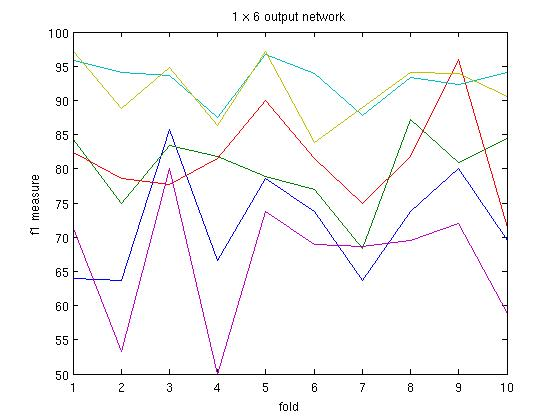
\includegraphics[width=\linewidth]{1by6plot.jpg}
\caption{"F1 performance for the 6 output network"}
\end{figure}
\begin{figure} [H]
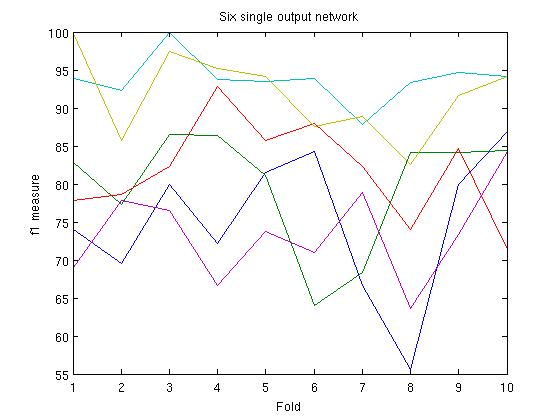
\includegraphics[width=\linewidth]{6by1plot.jpg}
\caption{"F1 performance for the single output networks"}
\end{figure}


\section{Implementation Details}
% Brief summary of implementation details (e.g., (e.g., how you performed cross-validation,
% how you classified each example based on %the 6 outputs, 
%anything that you think it is important in your system implementation);
\section{Questions}

\subsection{Discuss how you obtained the optimal topology and optimal values of network parameters. Describe the performance measure you used (and explain why you preferred it over other measures) and the different topologies / parameters you experimented with}
%Question above /\

%FIKSEN/GIO/ME first part (optimal topology/values)

%GIO talk about f1 vs other measures please

We experimented with the following parameters
\begin{enumerate}
  \item Number of hidden layers
  \item Number of hidden neurons in each layer
  \item Transfer function
  \item Training function
  \item Learning rate \emph{(where appropriate)}
  \item Momentum \emph{(where appropriate)}
\end{enumerate}

We decided to make the search space for (1) between 1 - 2. We took this decision as the lecture notes indicate "Networks with many hidden layers are prone to overfitting and harder to train, for most problems one hidden layer should be enough, 2 hidden layers can sometimes lead to improvement". Further to this, the course textbook claims that few practical applications ever need 3 or more layers.

Initially We decided to make the search space for (2) between 1-17 neurons for layer 1, 0 - 30 for layer 2 (0 layer 2 neurons representing only 1 layer in NN). We got these values through researching NNs and found these quotes by Jeff Heaton in \emph{Introduction to Neural Networks In Java} -- "the optimal size of the hidden layer is usually between the size of the input and size of the output layers" and "A good number of neurons is likely to be around the average of the inputs and outputs". We then experimented, varying the layer sizes and observed when the number of neurons > 30, training time simply far surpassed any improvement and therefore we made this the ceiling.

The number of layers and neurons/layer were initially calculated using a brute force method in which we went through every combination of layer 1 and layer 2 neurons in the search space and calculated the average f1 measure for each network (keeping default values for transfer functions etc.). The results of running this brute force test can be seen in the graphs below. This gave us the conclusion that the topology [13,27] was the best with other default parameters, and gave us a seed value for later.

[INSERT graphs here]

Having tested optimal topology using brute force, we decided to use a more elegant solution to get us our final optimal network by using a genetic algorithm.

For this algorithm to run in enough time to complete the project, we noticed we would have to drastically reduce the search space. As such, we decided to remove a large number of in built training functions as they were unnecessary, slow or incompatible with our NN.
We limited out search space to the following transfer functions:
\begin{multicols}{2}
\begin{itemize}
  \item trainbfg
  \item traincgb
  \item traincgf
  \item traincgp
  \item traingda
  \item traingdm
  \item traingdx
  \item trainlm
  \item trainoss
  \item trainrp
  \item trainscg 
\end{itemize}
\end{multicols}

These were selected from a list of 20 functions taken from the Matlab NNToolbox documentation. We removed the training functions which weren't suitable for batch training and, after reading further into the documentation, we decided to not use 'trainb', 'traingd' and 'traigdm' - our justification being "The previous section presented two backpropagation training algorithms: gradient descent, and gradient descent with momentum. These two methods are often too slow for practical problems. In this section we discuss several high performance algorithms that can converge from ten to one hundred times faster than the algorithms discussed previously.".

There were a huge amount of parameters to the different transfer functions, so to simplify or searching, we decided to optimise only learning rate and 'mu' (momentum) which were allowed to take values between 0 and 1 as multiples of 0.1.

The transfer functions were also tested in the same manner.

After running the genetic algorithm for a population size of 100 over 100 generations we got 
what appears to be the optimal parameters.




%FIKSEN talk about the training functions/params

\subsection{Explain what strategy you employed to ensure good generalisation ability of the networks and overcome the problem of overfitting}

We optimised our networks based on the f1 measure for predictions of unseen target values, this would mean that overfitted networks should perform worse and be discarded by our genetic algorithm. To make our genetic algorithm faster we discarded networks which were likely to overfit the data by bounding some of the parameters. We made sure the number of neurons per level to above 5, so it could understand the data sufficiently, and below 30 so that it is not overfitted. We also restricted the number of epochs to 100 so that the network does not become too familiar to the data. 

\subsection{In Part VIII you used the optimal parameters that you found in part VI to train your networks. However, there is a problem with this approach, the data you used for validation at some point will be used for testing in cross-validation. Can you explain why this a problem? Ideally how should you optimise the parameters in cross-validation?}

We were given a number of examples and targets we then divided these into  2/3 training and 1/3 validation data. The validation data then influences the neural network which is produced. Essentially you are training the neural network to perform well for the validation data and you hope that the validation data is large and representitive enough so that the neural network you produce generalises well and can classify unseen examples. When you come to perform cross validation you then use a portion of the data as testing data and the rest as training/validation data. This means that eventually you will be testing a section of data which was the network was geared for this will produce a very low error and thus will skew the average error rate affecting your cross validation result. To combat this the parameters (data) given to cross validation should be rearranged into a random order this will reduce the effect of any 'seen' data and any effects will be evenly spread and the average will not be skewed, althought it could be raised very slightly.

\subsection{Is there any difference in the classification performance of the two different classification approaches. Discuss the advantages / disadvantages of using 6 single-outut NNs vs. 1 six-output NNs}

Six single output neural networks perform much better than a single network. 

The six networks have the advantage of collectively forming a larger, more complicated and understanding, network without overfitting individually. The isolation between the networks allows for parallelism and for greater parameter specialisation for different emotions. One disadvantage is that having multiple networks may introduce merging conflicts when resolving an answer. This could be solved by limiting outputs to continuous output so that results are very unlikely to match or by ranking networks based on reliability, for example f1 measure, classification rate, most general/simple (i.e. fewer neurons), which also adds to the processing.

The single network however forms a smaller network which is less memory intensive and quicker to train and run. This means more aggressive optimisations can be performed resulting in parameters which are more finely tuned. This network would be more suited for machines whrecomputing resources are limited.

\section{Code Flow Charts}

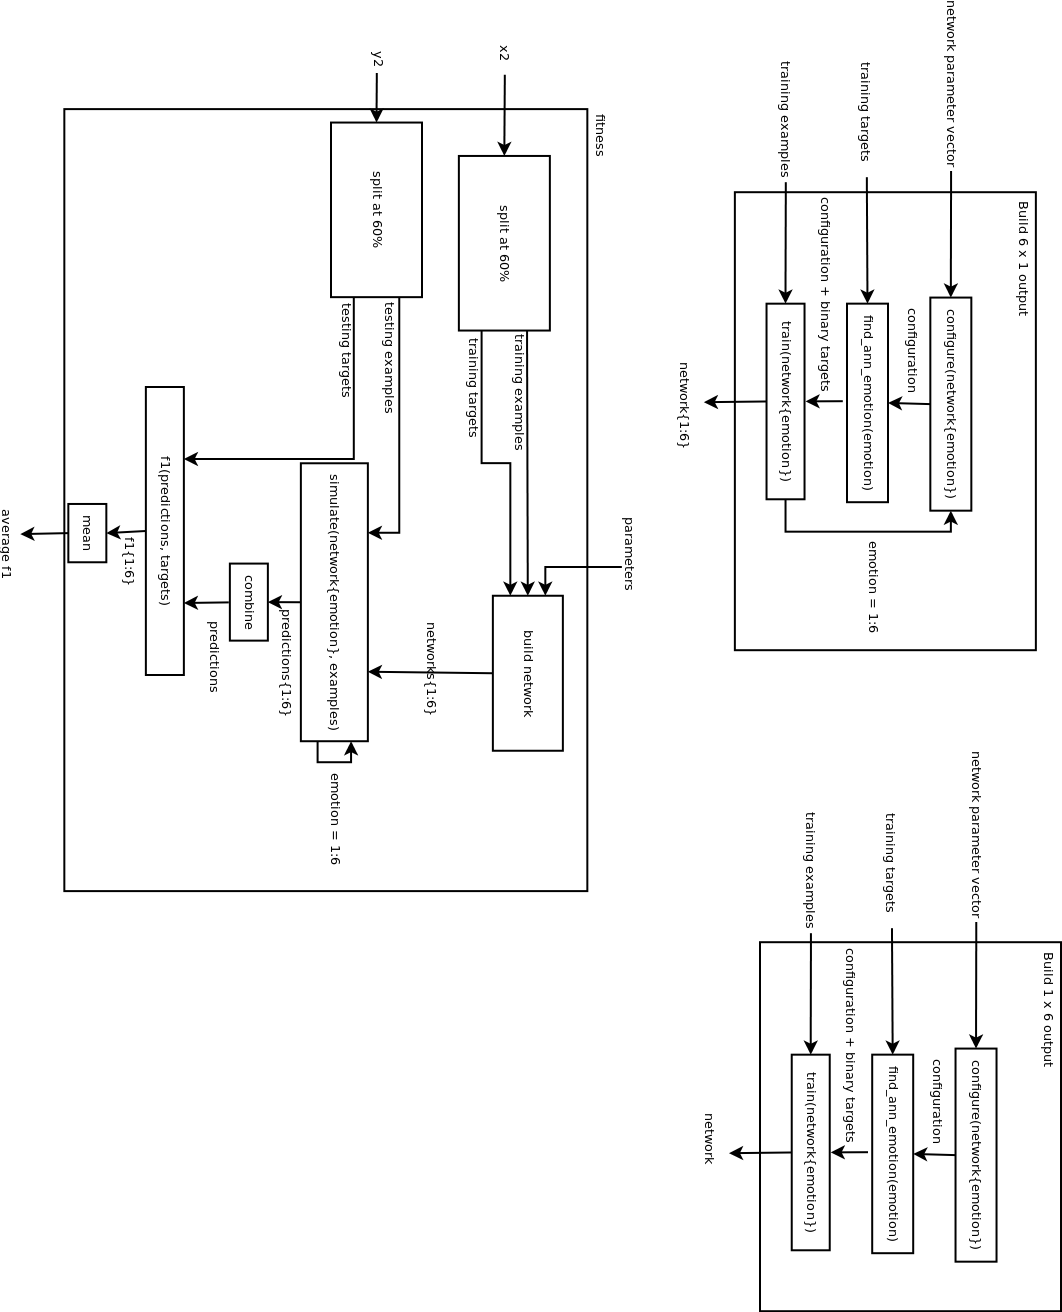
\includegraphics[width=\linewidth]{build_networks.png}
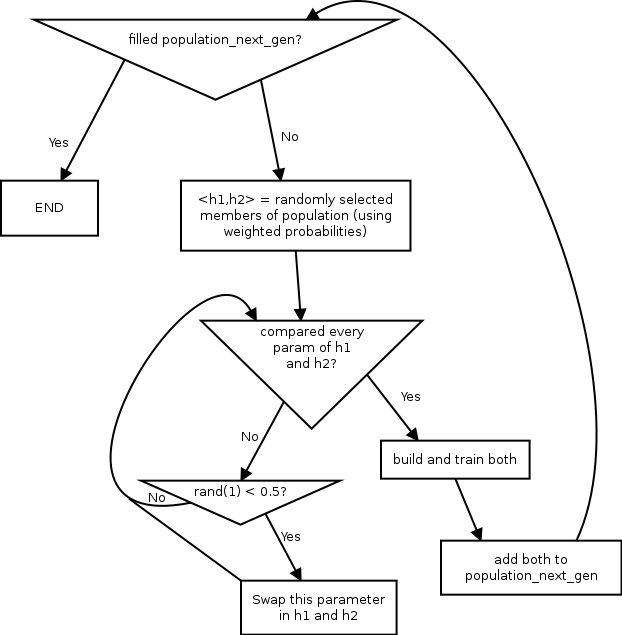
\includegraphics[width=\linewidth]{crossover.png}
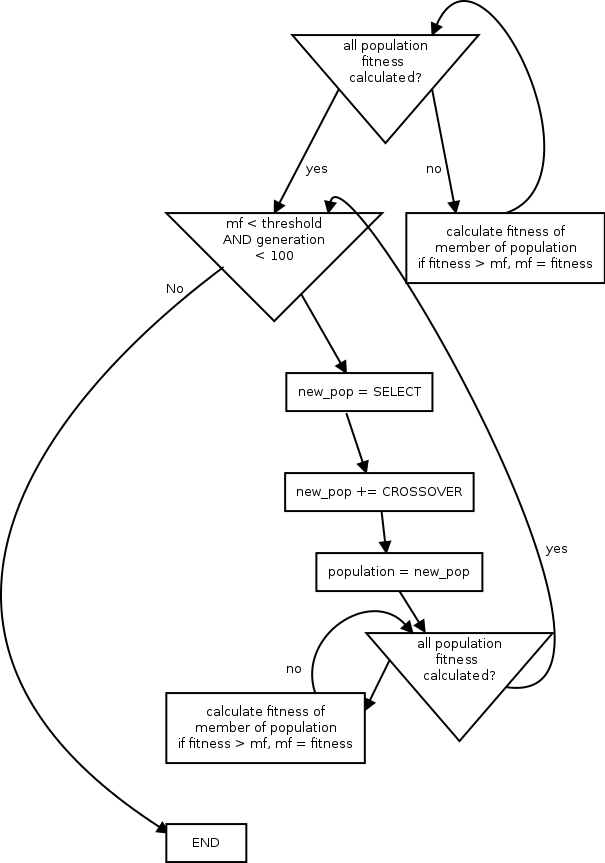
\includegraphics[width=\linewidth]{genetic_algorithm_diagram.png}
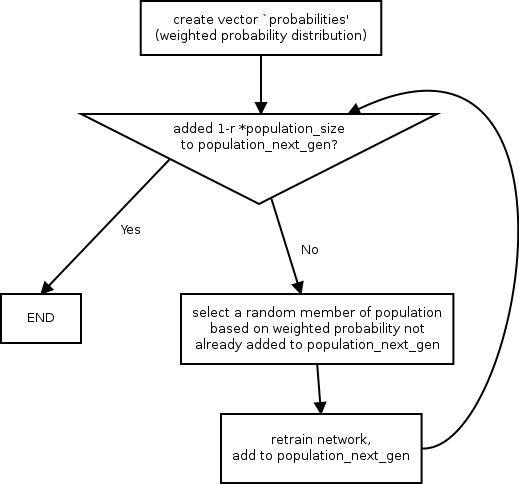
\includegraphics[width=\linewidth]{select.png}


\end{document}
